\documentclass[10pt]{beamer}
\usepackage[frenchb]{babel}
\usepackage[T1]{fontenc}
\usepackage[utf8]{inputenc}
\usetheme{metropolis}
\usepackage{appendixnumberbeamer}
\usepackage{csquotes} %guillemets
\usepackage{graphicx}
\usepackage{booktabs}
\usepackage{mathtools}
\usepackage{epigraph}
\usepackage{listings}
\usepackage[scale=2]{ccicons}

\usepackage{pgfplots}
\usepackage[absolute,overlay]{textpos}
\usepgfplotslibrary{dateplot}

\usepackage{soul}

\usepackage{xspace}
\newcommand{\themename}{\textbf{\textsc{metropolis}}\xspace}

\author{Matthieu NICOLAS}
\title{(Ré)Identification efficace dans les types de données répliquées sans conflit (CRDTs)}
%\institute{\includegraphics[scale=0.2]{fig/ul-logo.pdf}\hspace{0.3em}University of Lorraine $|$ \includegraphics[scale=0.08]{fig/inria-logo.pdf}\hspace{0.3em}COAST team $|$ OpenPaaS project\newline \includegraphics[scale=0.2]{fig/supervision-text.pdf}}
\date{Juin 2017}

\begin{document}

\begin{frame}[t,plain]
\titlepage
\end{frame}

\begin{frame}{Déroulement de carrière}
  \begin{center}
    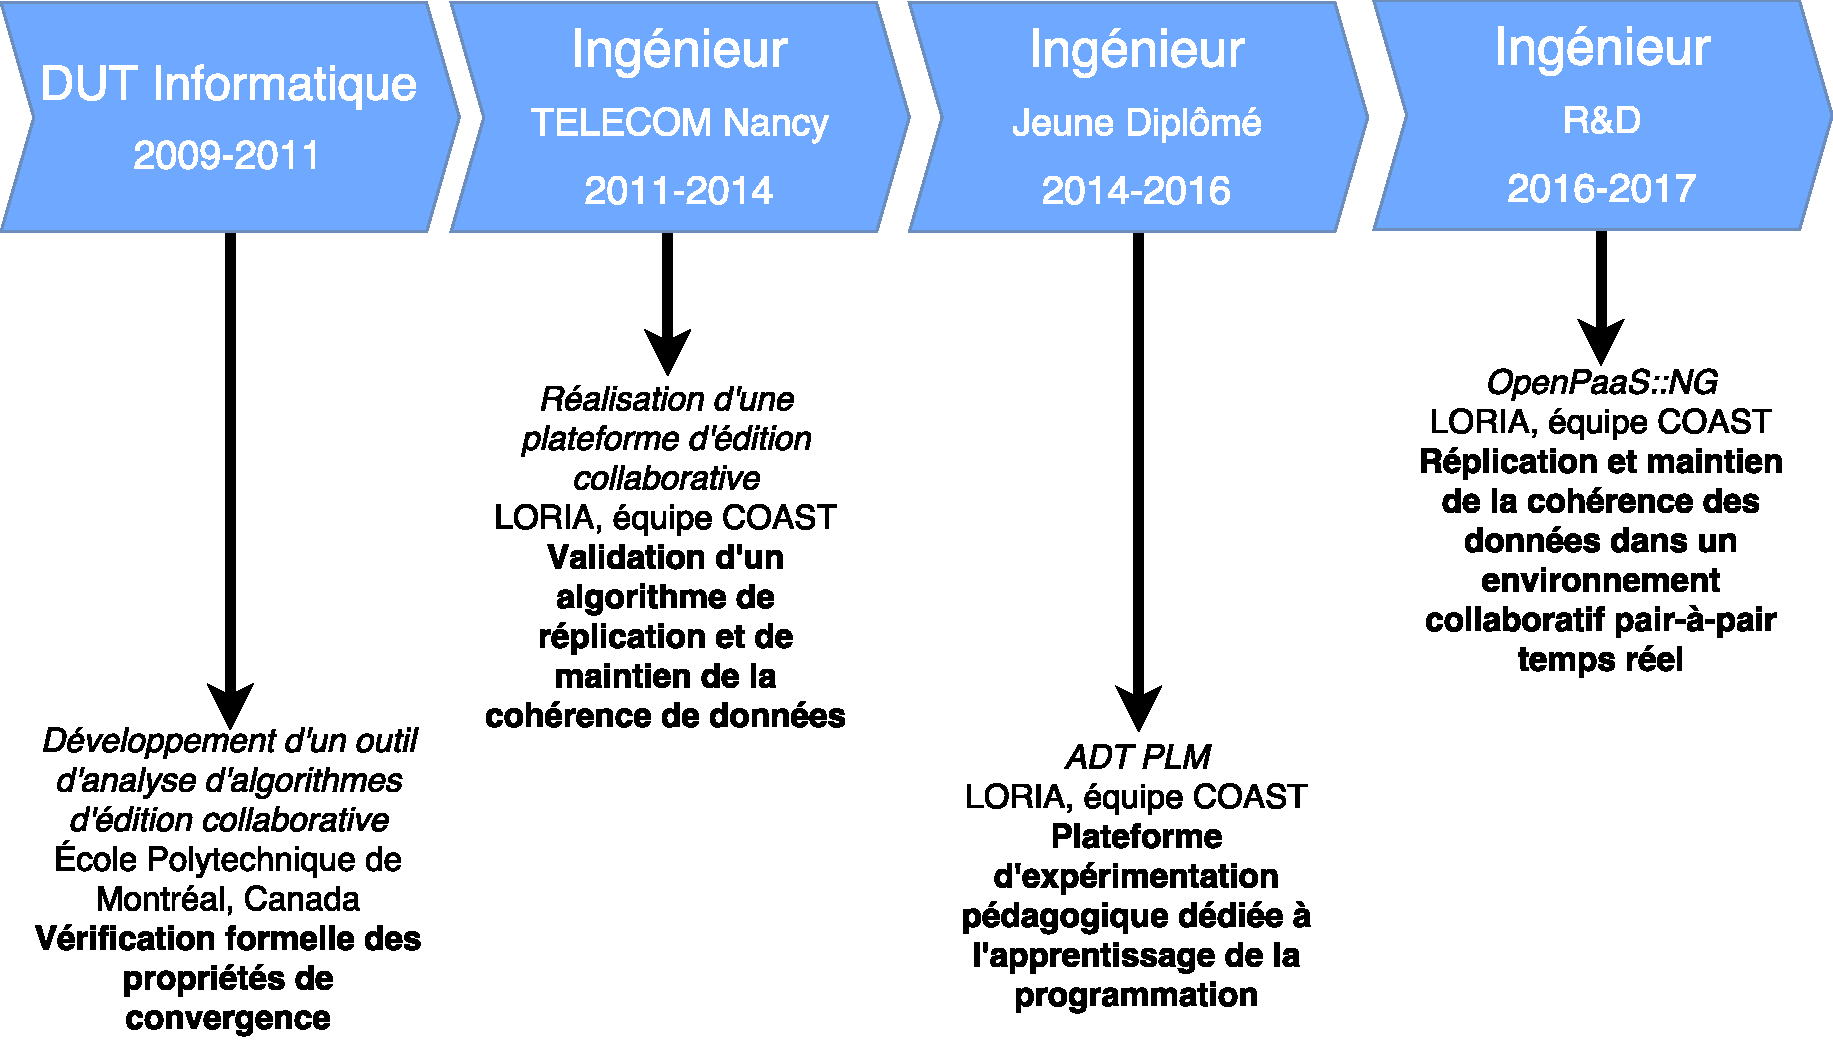
\includegraphics[scale=0.35]{fig/frise.pdf}
  \end{center}
\end{frame}

\begin{frame}{3 ans d'expériences en milieu académique}
  \begin{center}
    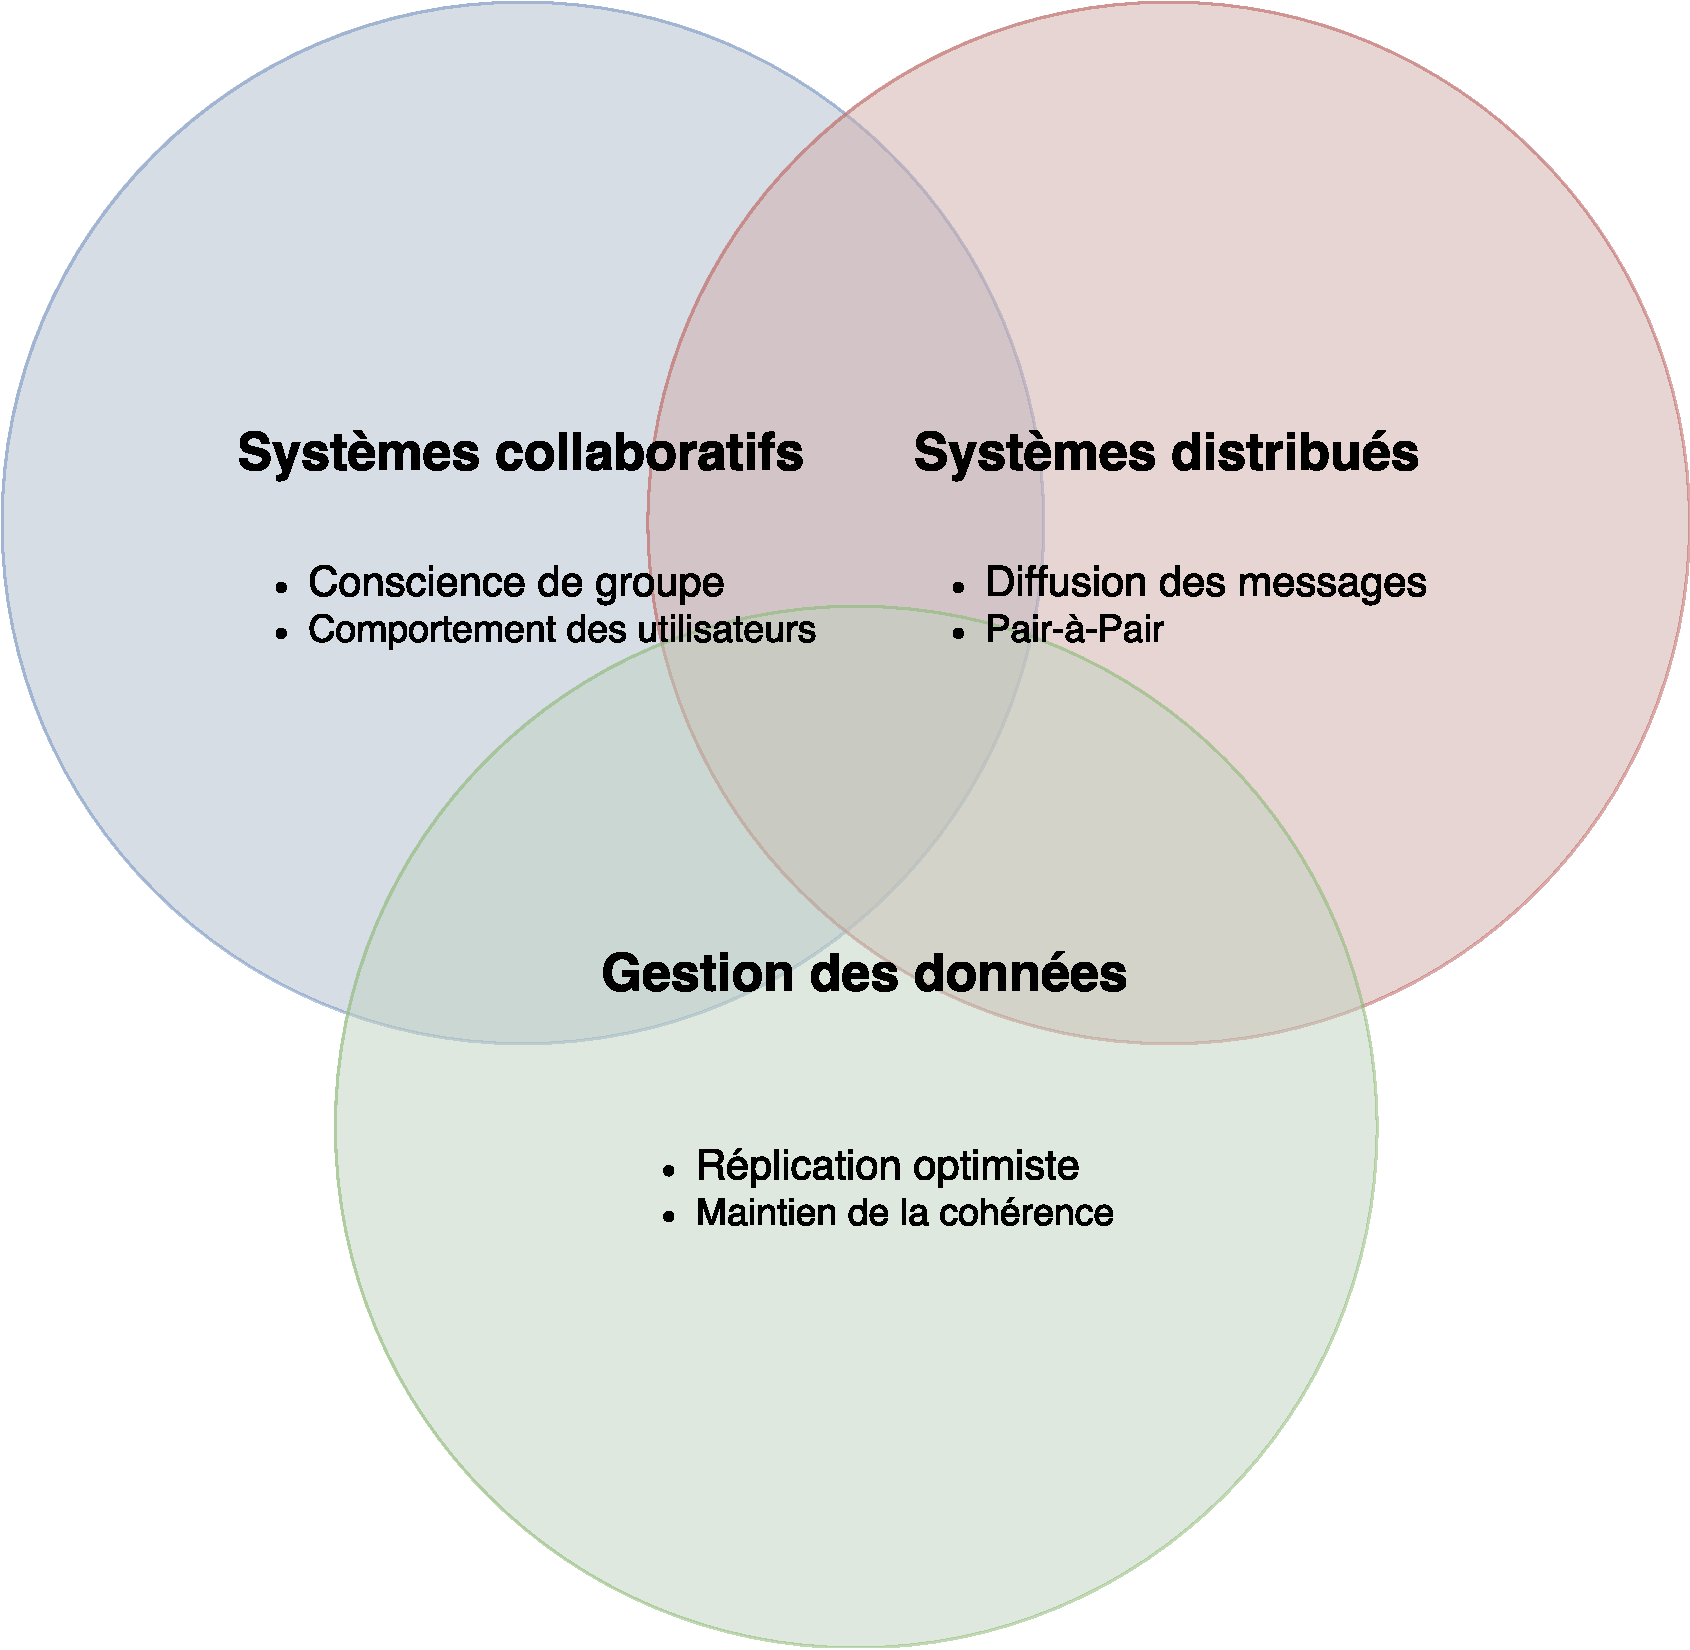
\includegraphics[scale=0.25]{fig/patates.pdf}
  \end{center}
\end{frame}

%\begin{frame}{... dans une équipe de recherche}
%  \begin{itemize}
%    \item 3 ans dans une équipe de recherche
%    \item Échange au quotidien avec des chercheurs, des doctorants...
%  \end{itemize}
%\end{frame}

\begin{frame}{Motivations}
  \begin{itemize}
    \item Projet professionnel : \textbf{carrière académique}
    \item Choix réfléchi
    \item Thématique de recherche :
      \begin{itemize}
        \item \st{Apprentissage automatique (\emph{lifelong machine learning})}
        \item Systèmes distribués / réplication / cohérence des données
      \end{itemize}
  \end{itemize}
\end{frame}

\begin{frame}{(Ré)Identification efficace dans les CRDTs}
  \begin{itemize}
    \item Contexte
    \begin{itemize}
      \item Réplication de données dans les systèmes distribués
      \item Approche des types de données répliquées sans conflit \cite{ShapiroSSS2011}
    \end{itemize}

    \item Problématique : gestion des identifiants

    \item Rôle des identifiants
    \begin{itemize}
      \item Identifie de façon unique : \textbf{Unicité}
      \item Indique la causalité des opérations : \textbf{Relation d'ordre}
      \item Ordonne les éléments (structure linéaire) : \textbf{Espace dense}
    \end{itemize}

    \begin{itemize}
      \item Taille non-bornée des identifiants
      \item Accroissement de la part de méta-données à stocker et échanger
    \end{itemize}

%    \item Contraintes du système
%    \begin{itemize}
%      \item Haute disponibilité
%      \item Tolérance aux partitionnement
%      \item Préservation de l'intention
%    \end{itemize}

%    \item Besoin de généraliser aux autres CRDTs

  \end{itemize}
\end{frame}

\begin{frame}[standout]
  Merci pour votre attention, avez-vous des questions ?
\end{frame}

\begin{frame}[allowframebreaks]{References}
	\bibliography{biblio}
	\bibliographystyle{abbrv}
\end{frame}


\end{document}
